\let\negmedspace\undefined
\let\negthickspace\undefined
\documentclass[journal,12pt,onecolumn]{IEEEtran}
\usepackage{cite}
\usepackage{amsmath,amssymb,amsfonts,amsthm}
\usepackage{amsmath}
\usepackage{algorithmic}
\usepackage{graphicx}
\usepackage{textcomp}
\usepackage{circuitikz}
\usepackage{xcolor}
\usepackage{txfonts}
\usepackage{listings}
\usepackage{multicol}
\usepackage{enumitem}
\usepackage{mathtools}
\usepackage{gensymb}
\usepackage{comment}
\usepackage[breaklinks=true]{hyperref}
\usepackage{tkz-euclide} 
\usepackage{listings}
\usepackage{gvv}                                        
\usepackage[latin1]{inputenc}                                
\usepackage{color}                                            
\usepackage{array}                                            
\usepackage{longtable}                                       
\usepackage{calc}                                             
\usepackage{multirow}                                         
\usepackage{hhline}                                           
\usepackage{ifthen}                                           
\usepackage{lscape}
\usepackage{tabularx}
\usepackage{array}
\usepackage{float}


\newtheorem{theorem}{Theorem}[section]
\newtheorem{problem}{Problem}
\newtheorem{proposition}{Proposition}[section]
\newtheorem{lemma}{Lemma}[section]
\newtheorem{corollary}[theorem]{Corollary}
\newtheorem{example}{Example}[section]
\newtheorem{definition}[problem]{Definition}
\newcommand{\BEQA}{\begin{eqnarray}}
\newcommand{\EEQA}{\end{eqnarray}}
\newcommand{\define}{\stackrel{\triangle}{=}}
\theoremstyle{remark}
\newtheorem{rem}{Remark}

\begin{document}
\bibliographystyle{IEEEtran}
\vspace{3cm}

\title{2010-PH-40-52}
\author{EE24BTECH11001 -  ADITYA TRIPATHY}
\maketitle

\renewcommand{\thefigure}{\theenumi}
\renewcommand{\thetable}{\theenumi}

\begin{enumerate}
    \item[40.] The figure shows a current source charging a capacitor that is initially uncharged
        \begin{center}
            \resizebox{0.2\textwidth}{!}{%
                \begin{circuitikz}
                    \tikzstyle{every node}=[font=\LARGE]
                    \draw (7.5,16.5) to[american current source] (7.5,18.75);
                    \draw (7.5,16.5) to (7.5,14.75) node[ground]{};
                    \draw (7.5,18.75) to[short] (9.5,18.75);
                    \draw (9.5,18.75) to[normal open switch] (11.5,18.75);
                    \draw (11.5,18.75) to[C] (11.5,16.75);
                    \draw (11.5,16.75) to (11.5,14.75) node[ground]{};
                \end{circuitikz}
                }
        \end{center}
        If the switch is closed at $t = 0$, which of the following plots depicts correctly the output
        voltage of the circuit as a function of time?
        \hfill{\brak{2010-PH}}
        \begin{enumerate}
                \begin{multicols}{2}
                \item  
                    \begin{center}
                        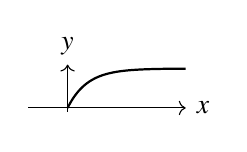
\begin{tikzpicture}[scale = 0.5]
                            % Draw axes
                            \draw[->] (-1,0) -- (3,0) node[right] {$x$}; % x-axis
                            \draw[->] (0,-0.1) -- (0,1.1) node[above] {$y$}; % y-axis

                            % Draw the function y = 1 - e^(-2x)
                            \draw[black, thick, domain=0:3, samples=100] plot (\x, {1 - exp(-2*\x)});
                        \end{tikzpicture}
                    \end{center}

                    \columnbreak
                \item 
                    \begin{center}
                        \begin{tikzpicture}[scale = 0.5]
                            % Draw axes
                            \draw[->] (-1,0) -- (3,0) node[right] {$t$}; % x-axis
                            \draw[->] (0,-2) -- (0,2) node[above] {$V_{\text{out}}$}; % y-axis

                            % Draw the function y = -5x(x-2)
                            \draw[black, thick, domain=0:2, samples=100] plot (\x, {-1 * \x*(\x-2)});

                        \end{tikzpicture}               
                    \end{center}
                \end{multicols}
                \begin{multicols}{2}

                \item 
                    \begin{center}
                        \begin{tikzpicture}[scale=0.5]
                            % Draw axes
                            \draw[->] (-2,0) -- (6,0) node[right] {$t$}; % x-axis
                            \draw[->] (0,-2) -- (0,3) node[above] {$V_{\text{out}}$}; % y-axis

                            % Draw the line y = x
                            \draw[black, thick] (0,0) -- (3,3);
                            \draw[thick] (3,3) -- (5,3);
                        \end{tikzpicture}
                    \end{center}
                    \columnbreak
                \item
                    \begin{center}
                        \begin{tikzpicture}[scale=0.5]
                            \draw[->] (0,0) -- (4,0) node[right] {$t$};
                            \draw[->] (0,0) -- (0,2.5) node[left] {$V_{out}$};

                            % The curve
                            \draw[thick] (0.8,0) .. controls(1,0.2) .. (1,0.2) to[out=60,in=180] (2,2) ;

                        \end{tikzpicture}
                    \end{center}

                \end{multicols}
        \end{enumerate}
    \item[41.] For any set of inputs, $A$ and $B$, the following circuits give the same output , $Q$, except
        one. Which one is it?

        \hfill{\brak{2010-PH}}
        \begin{enumerate}
                \begin{multicols}{2}

                \item  

                    \begin{center}

                        \resizebox{0.3\textwidth}{!}{%
                            \begin{circuitikz}
                                \tikzstyle{every node}=[font=\LARGE]
                                \draw (7.5,15.5) to[short] (7.75,15.5);
                                \draw (7.5,15) to[short] (7.75,15);
                                \draw (7.75,15.5) node[ieeestd xor port, anchor=in 1, scale=0.89](port){} (port.out) to[short] (9.5,15.25);
                                \draw (5.75,15.5) to[short] (7.75,15.5);
                                \draw (5.75,15) to[short] (7.75,15);
                                \draw (6.75,13.25) to[short] (6.75,15);
                                \draw (6.75,13.25) to[short] (9.5,13.25);
                                \draw (9.75,13.25) node[ieeestd not port, anchor=in](port){} (port.out) to[short] (11.5,13.25);
                                \draw (port.in) to[short] (9.5,13.25);
                                \draw (9.5,15.25) to[short] (11.5,15.25);
                                \draw (11.5,15.25) to[short] (13.5,15.25);
                                \draw (11.5,13.25) to[short] (11.5,14.75);
                                \draw (11.5,14.75) to[short] (13.5,14.75);
                                \draw (13.5,15.25) to[short] (13.75,15.25);
                                \draw (13.5,14.75) to[short] (13.75,14.75);
                                \draw (13.75,15.25) node[ieeestd and port, anchor=in 1, scale=0.89](port){} (port.out) to[short] (15.5,15);
                            \end{circuitikz}
                            } 
                    \end{center}
                    \columnbreak
                \item 
                    \begin{center}

                        \resizebox{0.3\textwidth}{!}{%
                            \begin{circuitikz}
                                \tikzstyle{every node}=[font=\LARGE]
                                \draw (10.25,16.75) to[short] (10.5,16.75);
                                \draw (10.25,16.25) to[short] (10.5,16.25);
                                \draw (10.5,16.75) node[ieeestd and port, anchor=in 1, scale=0.89](port){} (port.out) to[short] (12.25,16.5);
                                \draw (8.5,16.25) node[ieeestd not port, anchor=in](port){} (port.out) to[short] (10.25,16.25);
                                \draw (port.in) to[short] (8.25,16.25);
                                \draw (8,16.75) to[short] (10,16.75);
                                \draw (8.5,16.75) to[short] (10.5,16.75);
                            \end{circuitikz}
                            }

                    \end{center}

                \end{multicols}
                \begin{multicols}{2}

                \item
                    \begin{center}
                        \resizebox{0.3\textwidth}{!}{%
                            \begin{circuitikz}
                                \tikzstyle{every node}=[font=\LARGE]
                                \draw (13,18.25) to[short] (13.25,18.25);
                                \draw (13,17.75) to[short] (13.25,17.75);
                                \draw (13.25,18.25) node[ieeestd and port, anchor=in 1, scale=0.89](port){} (port.out) to[short] (15,18);
                                \draw (11.25,17.75) node[ieeestd not port, anchor=in](port){} (port.out) to[short] (13,17.75);
                                \draw (port.in) to[short] (11,17.75);
                                \draw (9,18.75) to[short] (13,18.75);
                                \draw (13,18.25) to[short] (13,18.75);
                                \draw (9,17.75) to[short] (11,17.75);
                                \draw (10,16.25) to[short] (10,18.75);
                                \draw (13,16.75) to[short] (13.25,16.75);
                                \draw (13,16.25) to[short] (13.25,16.25);
                                \draw (13.25,16.75) node[ieeestd and port, anchor=in 1, scale=0.89](port){} (port.out) to[short] (15,16.5);
                                \draw (10,16.25) to[short] (13,16.25);
                                \draw (13,16.75) to[short] (13,17.75);
                                \draw (15,16.5) to[short] (15.25,16.5);
                                \draw (15,16) to[short] (15.25,16);
                                \draw (15.25,16.5) node[ieeestd and port, anchor=in 1, scale=0.89](port){} (port.out) to[short] (17,16.25);
                                \draw (15,16) to[short] (15,15.25);
                                \draw (15,15.25) to[short] (11,15.25);
                                \draw (11,15.25) to[short] (11,17.75);
                                \draw (17,18) to[short] (17.25,18);
                                \draw (17,17.5) to[short] (17.25,17.5);
                                \draw (17.25,18) node[ieeestd or port, anchor=in 1, scale=0.89](port){} (port.out) to[short] (19,17.75);
                                \draw (17,16.25) to[short] (17,17.5);
                                \draw (15,18) to[short] (17,18);
                            \end{circuitikz}
                            }
                    \end{center}

                    \columnbreak
                \item 
                    \begin{center}

                        \resizebox{0.3\textwidth}{!}{%
                            \begin{circuitikz}
                                \tikzstyle{every node}=[font=\LARGE]
                                \draw (13.25,17.5) to[short] (13.5,17.5);
                                \draw (13.25,17) to[short] (13.5,17);
                                \draw (13.5,17.5) node[ieeestd or port, anchor=in 1, scale=0.89](port){} (port.out) to[short] (15.25,17.25);
                                \draw (11.5,17.5) node[ieeestd not port, anchor=in](port){} (port.out) to[short] (13.25,17.5);
                                \draw (port.in) to[short] (11.25,17.5);
                                \draw (11.5,17) to[short] (13.5,17);
                                \draw (11.25,17) to[short] (13.25,17);
                            \end{circuitikz}
                            }
                    \end{center}

                \end{multicols}
            \end{enumerate}

        \item[42.] $CO_2$ molecule has the first few energy levels uniformly separated by approximately
            2.5 meV. At a temperature of $300K$, the ratio of the number of moleciles in the $4^{th}$
            excited state to the number in the $2^{nd}$ excited state is about 
            \hfill{\brak{2010-PH}}
            \begin{enumerate}
                \item 0.5
                \item 0.6
                \item 0.8
                \item 0.9
            \end{enumerate}

        \item[43.] Which among the following sets of Maxwell relations is correct? $\brak{U -
            \textnormal{internal energy},\\ H - \textnormal{enthalpy}, A - \textnormal{Helmholtz free energy},
            G - \textnormal{Gibbs free energy}}$ 

            \hfill{\brak{2010-PH}}
            \begin{enumerate}
                \item $T = \brak{\frac{\partial U}{\partial V}}_S$ and  $P = \brak{\frac{\partial U}{\partial S}}_V$
                \item $V = \brak{\frac{\partial H}{\partial P}}_S$ and  $T = \brak{\frac{\partial H}{\partial S}}_P$
                \item $P = -\brak{\frac{\partial G}{\partial V}}_T$ and  $V = \brak{\frac{\partial G}{\partial P}}_S$
                \item $T = -\brak{\frac{\partial A}{\partial S}}_T$ and  $V = \brak{\frac{\partial G}{\partial P}}_S$
            \end{enumerate}

        \item[44.] For a spin-s particle, the the eigen basis of $\bar{S}.S$, the expectation value
            $\langle \; sm|S^2,|sm \; \rangle$ is

            \hfill{\brak{2010-PH}}
            \begin{enumerate}
                \item $\frac{\hbar ^ 2 \cbrak{s\brak{s + 1} - m^2}}{2}$
                \item $\hbar ^ 2 \cbrak{s\brak{s + 1} - 2m^2}$
                \item $\hbar ^ 2 \cbrak{s\brak{s + 1} - m^2}$
                \item $\hbar ^2 m^2$
            \end{enumerate}

        \item[45.] A particle is placed in a region with potential $V\brak{x} = \frac{1}{2}kx^2 - 
            \frac{\lambda}{3}x^2$, where $k, \lambda > 0$. Then,
            \hfill{\brak{2010-PH}}
            \begin{enumerate}
                \item $x = 0$ and $x = \frac{k}{\lambda}$ are points of stable equilibrium
                \item $x = 0$ is a point of stable equilibrium and  $x = \frac{k}{\lambda}$ is a point of unstable equilibrium
                \item $x = 0$ and $x = \frac{k}{\lambda}$ are points of unstable equilibrium
                \item There are no points of stable or unstable equilibrium
            \end{enumerate}
        \item[46.] A $\pi$ meson at rest decays into two photons, which move along $x$-axis. They are
            both detected simultaneously after time, $t = 10s$. In an inertial frame moving with velocity 
            $V = 0.6c$ in the direction of one of the photons, the interval between the two detections is
            \hfill{\brak{2010-PH}}
            \begin{enumerate}
                \item 15s
                \item 0s
                \item 10s
                \item 20s
            \end{enumerate}

        \item[47.] A particle of mass $m$ is confined in an infinite potential well:
            \begin{align}
                V\brak{x} =  \begin{cases}
                    0 & \textnormal{if}  \quad 0 < x < L,\\
                    \infty & \textnormal{otherwise}
                \end{cases}
            \end{align}
            It is subjected to a perturbing potential $V_p = V_o \sin \brak{\frac{2\pi x}{L}}$
            within the well. Let $E^1$ and $E^2$ be the corrections to the ground state energy in the 
            first and second order in $V_0$, respectively. Which of the following are true
            \hfill{\brak{2010-PH}}
            \begin{enumerate}
                \item $E^1 = 0, E^2 < 0$
                \item $E^1>0, E^2 = 0$
                \item $E^1 = 0, E^2$ depends in the sign of $V_0$
                \item $E^1 < 0, E^2 < 0$
            \end{enumerate}
            \section{\textbf{Common Data Questions}}
            \textbf{Common Data for Questions 48 and 49}\\
            In the presence of a weak magnetic field, atomic hydrogen undergoes the transition :
            \begin{align}
                {\quad}^2 P_{\frac{1}{2}} \rightarrow {\quad}^1 S_{\frac{1}{2}}
            \end{align}
            by the emmision of radiation.
        \item[48.] The number of lines that are observed in the Zeeman spectrum is
            \hfill{\brak{2010-PH}}
            \begin{enumerate}
                \item 2
                \item 3
                \item 4
                \item 6
            \end{enumerate}
        \item[49.] The spectral line corresponding to the transition 
            \begin{align}
                {\quad}^2 P_{\frac{1}{2}}\brak{m_j = + \frac{1}{2}} \rightarrow {\quad}^1 S_{\frac{1}{2}}\brak{m_j = -\frac{1}{2}}
            \end{align}
            is observed along the direction of the applied magnetic field. The emitted electromagnetic
            field is
            \hfill{\brak{2010-PH}}
            \begin{enumerate}
                \item Circularly polarized
                \item Linearly polarized
                \item unpolarized
                \item Not emitted along the magnetic field direction
            \end{enumerate}
            \textbf{Common Data for Questions 50 and 51}\\
            The partition function for a gas of photons is given by
            \begin{align}
                \ln Z = \frac{\pi^2 V\brak{k_B T}^3}{45\hbar ^3 C^3}
            \end{align}
        \item[50.] The specific heat of the photon gas varies with temperature as 
            \hfill{\brak{2010-PH}}
            \begin{enumerate}
                    \begin{multicols}{2}
                
                \item 
                    \begin{center}
                        \begin{tikzpicture}[scale = 0.5]
                            % Draw the axes
                            \draw[->] (0,0) -- (3,0) node[right] {$T$};
                            \draw[->] (0,0) -- (0,3) node[above] {$C_v$};

                            % Draw the function y = 0.5x^2
                            \draw[domain=0:2,smooth,variable=\x,black] plot ({\x},{0.5*\x*\x});
                        \end{tikzpicture}
                    \end{center}
                    \columnbreak
                \item 
                    \begin{center}
                        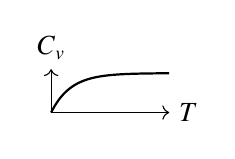
\begin{tikzpicture}[scale = 0.5]
                            % Draw axes
                            \draw[->] (0,0) -- (3,0) node[right] {$T$}; % x-axis
                            \draw[->] (0,0) -- (0,1.1) node[above] {$C_v$}; % y-axis

                            % Draw the function y = 1 - e^(-2x)
                            \draw[black, thick, domain=0:3, samples=100] plot (\x, {1 - exp(-2*\x)});
                        \end{tikzpicture}
                    \end{center}
            \end{multicols}
                    \begin{multicols}{2}
                
                \item 
                    \begin{center}
                        \begin{tikzpicture}[scale = 0.5]
                            % Draw the axes
                            \draw[->] (0,0) -- (3,0) node[right] {$T$};
                            \draw[->] (0,0) -- (0,3) node[above] {$C_v$};

                            % Draw the function y = 1/x
                            \draw[domain=0.35:3.2,smooth,variable=\x,black] plot ({\x},{1/\x});
                        \end{tikzpicture}
                    \end{center}
                    \columnbreak
                \item 
                    \begin{center}
                        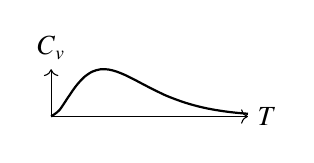
\begin{tikzpicture}[scale = 0.5]
                            % Draw the axes
                            \draw[->] (0,0) -- (5,0) node[right] {$T$};
                            \draw[->] (0,0) -- (0,1.2) node[above] {$C_v$};

                            % Draw the Boltzmann distribution curve
                            \draw[domain=0:5,smooth,variable=\x,black,thick] plot ({\x},{5*\x*\x*exp(-1.5*\x)});
                        \end{tikzpicture}
                    \end{center}
            \end{multicols}
            \end{enumerate}

        \item[51.] The pressure of the photon gas is
            \hfill{\brak{2010-PH}}
            \begin{enumerate}
                \item $\frac{\pi^2 \brak{k_B T}^3}{15\hbar ^3 C^3}$
                \item $\frac{\pi^2 \brak{k_B T}^4}{8\hbar ^3 C^3}$
                \item $\frac{\pi^2 \brak{k_B T}^4}{45\hbar ^3 C^3}$
                \item $\frac{\pi \brak{k_B T}^\frac{3}{2}}{45\hbar ^3 C^3}$
            \end{enumerate}

            \section{\textbf{Linked Answer Questions}}
            \textbf{Statement for Linked Answer Questions 52 , 53}\\
            Consider the propagation of electromagnetic waves in a linear, homogeneous and isotropic
            material medium with the electric permittivity $\epsilon$ and magnetic permeability $\mu$.\\
        \item[52.] For a plane wave of angular frequency $\omega$ and propagation vector $\vec{k}$ propagating
            in the medium Maxwell's equations reduce to
            \hfill{\brak{2010-PH}}
            \begin{enumerate}
                \item $\vec{k}\cdot \vec{E} = 0, \vec{k}\cdot \vec{H}, \vec{k} \times \vec{E}=\omega\epsilon \vec{H}, \vec{k} \times \vec{H}=-\omega\mu\vec{E}$ 
                \item $\vec{k}\cdot \vec{E} = 0, \vec{k}\cdot \vec{H}, \vec{k} \times \vec{E}=-\omega\epsilon \vec{H}, \vec{k} \times \vec{H}=\omega\mu\vec{E}$ 
                \item $\vec{k}\cdot \vec{E} = 0, \vec{k}\cdot \vec{H}, \vec{k} \times \vec{E}=-\omega\mu \vec{H}, \vec{k} \times \vec{H}=\omega\epsilon\vec{E}$ 
                \item $\vec{k}\cdot \vec{E} = 0, \vec{k}\cdot \vec{H}, \vec{k} \times \vec{E}=\omega\mu \vec{H}, \vec{k} \times \vec{H}=-\omega\epsilon\vec{E}$ 
            \end{enumerate}

    \end{enumerate}
\end{document}
